\documentclass[aspectratio=169]{beamer}
\usepackage{amsmath,tikz,graphicx,beamerpkg}
\setbeamertemplate{navigation symbols}{}
\title{Synthetic scientific presentation fixture}
\begin{document}
\begin{frame}{Simulation $\rightarrow$ experiment $\rightarrow$ analysis}
  \centering
  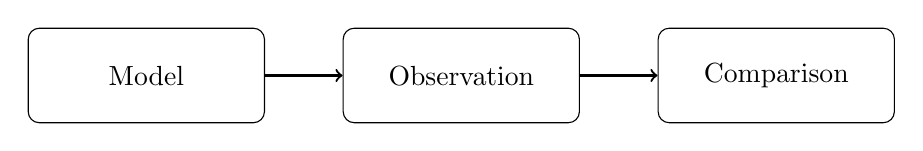
\begin{tikzpicture}[every node/.style={draw,rounded corners,minimum width=30mm,minimum height=12mm}]
    \node (s) at (0,0) {Model}; \node (e) at (4,0) {Observation}; \node (a) at (8,0) {Comparison};
    \draw[->,thick] (s)--(e); \draw[->,thick] (e)--(a);
  \end{tikzpicture}
  \par\bigskip A synthetic teaching example, not a validated scattering calculation.
\end{frame}
\begin{frame}{Scattering model: three overlays in one place}
  \begin{columns}
  \column{.5\textwidth}
  \[2d\sin\theta = n\lambda\]
  \uncover<2->{\[\mathbf{k}_{\mathrm{out}}-\mathbf{k}_{\mathrm{in}}=\mathbf{g}\]}
  \uncover<3->{\[I(\mathbf{q})\propto\left|\sum_j f_j e^{i\mathbf{q}\cdot\mathbf{r}_j}\right|^2\]}
  \column{.5\textwidth}
  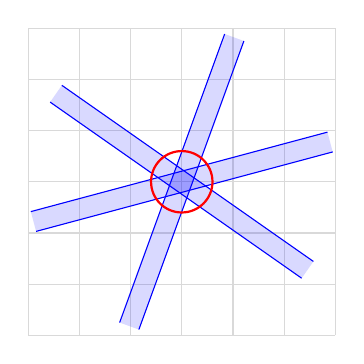
\begin{tikzpicture}[scale=.65]
  \draw[gray!30,step=1] (-3,-3) grid (3,3);
  \foreach \angle in {-35,15,70} {\begin{scope}[rotate=\angle]
    \fill[blue,opacity=.15] (-3,-.2) rectangle (3,.2);
    \draw[blue] (-3,-.2)--(3,-.2) (-3,.2)--(3,.2);
  \end{scope}}
  \only<3->{\draw[red,thick] (0,0) circle (.6);}
  \end{tikzpicture}
  \end{columns}
\end{frame}
\begin{frame}{Nearby experimental comparison}
  \begin{tikzpicture}
    \draw[->] (0,0)--(9,0) node[right] {$q$};
    \draw[->] (0,0)--(0,4) node[above] {$I$};
    \draw[blue,thick] plot[smooth] coordinates {(0,.2)(1,.3)(2,3)(3,.4)(4,.3)(5,2)(6,.2)(8,.1)};
    \foreach \x/\y in {1/.4,2/2.8,3/.5,4/.3,5/1.8,6/.4,8/.2} \fill[red] (\x,\y) circle (2pt);
  \end{tikzpicture}
  \par Synthetic curves and points used only to test presentation readability.
\end{frame}
\begin{frame}{Packaged observation: click to play}
  \centering\movie[loop,showcontrols]{\includegraphics[width=.65\textwidth]{media/video-poster_big.png}}{media/gemini_generated_video_b2693757.mp4}
\end{frame}
\begin{frame}{Packaged observation: autostart request}
  \centering\pkgpdfpcmovie[autostart&loop]{\includegraphics[width=.65\textwidth]{media/video-poster_big.png}}{media/gemini_generated_video_b2693757.mp4}
\end{frame}
\begin{frame}{Supplementary result for a temporary detour}
  \[\lim_{\mathbf{q}\to 0} e^{i\mathbf{q}\cdot\mathbf{r}} = 1\]
  \centering Escape returns to the saved guided overlay and camera.
\end{frame}
\end{document}
